\section{Introduction}
%RENAN - 1 pag

Hydropower has an important share in the global electricity production, and
will continue to be a major source of renewable power-generation\footnote{International Energy
Agency (2010), http://www.iea.org/.}% \cite{iea}.
. Large hydropower projects have typically an ave\-rage maintenance cost of 2\%
to 2.5\% of the investment cost per kW. A major maintenance concern
is the state of the runner's blades, which suffer cavitation and abrasion
phenomena. The erosion can lead to water flow instability, excessive vibrations
and turbine efficiency reduction \cite{goldemberg2007energia}, thus hard
coating techniques by thermal aspersion are used to greatly increase the life
cycle of runner's blades~\cite{krella2011new}.

The use of robotics for \textit{in situ} maintenance, and repair operations in
hydropower plants could greatly improve efficiency, health and safety, while
decreasing operational and logistical costs~\cite{hazel2012field}. The working
conditions on hydropower turbine installations are unfriendly, the atmospheric
conditions, high temperatures and humidity, and constrained space are
unfavorable to human operation (Fig.~\ref{fig::jirau_turb}). Also, some tasks,
as the hard coating procedure, require a robotic system due to high precision, speed, and the
usage of hazardous substances.

\begin{figure}[h!]
\centering
	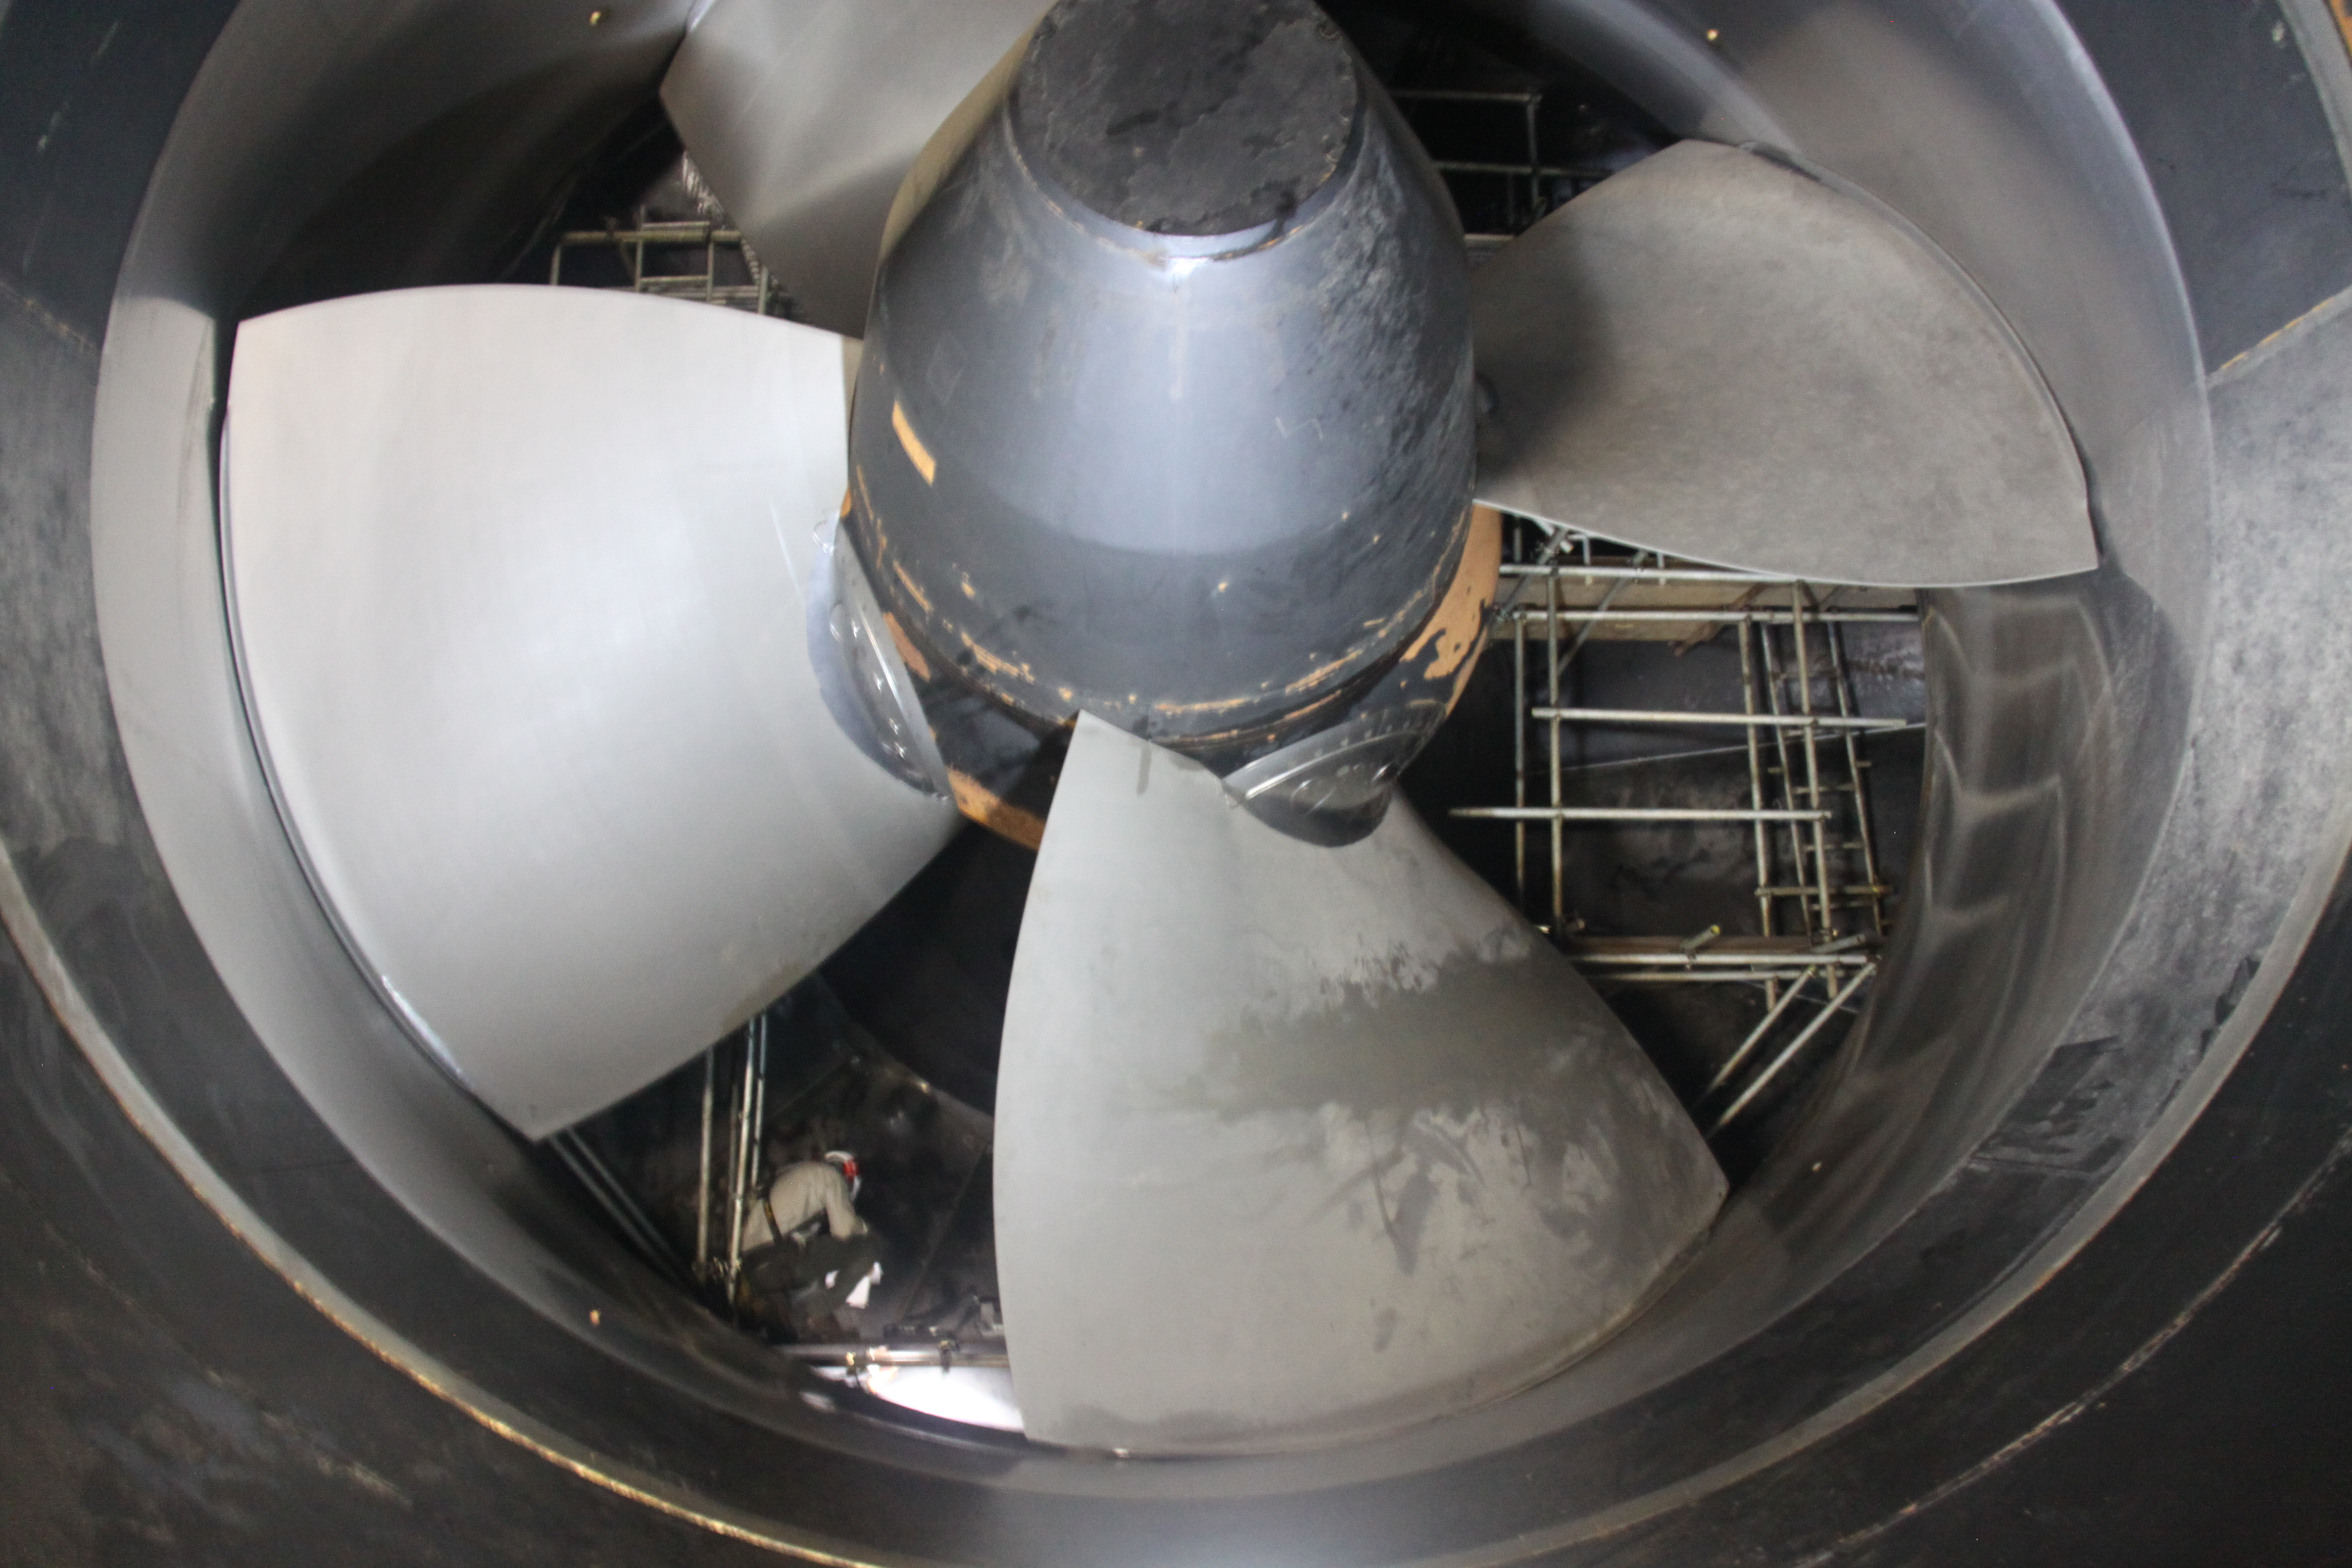
\includegraphics[width=\columnwidth]{figs/intro/jirau_turb.JPG} 
	\caption{Jirau's hydropower turbine.}
	\label{fig::jirau_turb}
\end{figure}

In the specific case of Brazil, hydropower is the largest
power-generation source. To support future economic growth, Brazil has
invested in additional large hydroelectric facilities, for instance, the
14~GW Belo Monte along the Xingu River\footnote{Energy
Information Administration (2014), https://www.eia.gov/.}%~\cite{eia}
, and Jirau dam
along the Madeira river. At the latter, the high concentration of suspended
particles carried by the river intensifies the abrasion phenomena, thus
regular maintenance is needed. 

Currently, blade coating maintenance in these large facilities is performed
before turbine assembling by a large-sized robotic manipulator, i.e., it is an
\textit{ex situ} process. \textit{In situ} maintenance would require robotic
system transportation, locomotion, placement and calibration. The majority of
the robotic systems for \textit{in situ} hydropower maintenance are used for
repair tasks, such as inspection, welding, and grinding. Some examples found in
the literature are:

\begin{itemize}
\item The Roboturb~\cite{roboturb} and the Scompi~\cite{scompi} are robotic
systems to perform erosion inspection and welding on damaged runner's blades.
They move on a flexible rail, which may be shaped and then fixed to the blade
surface.

\item \textit{The Climber}\footnote{International Climbing Machines (2013),
http://www.icm.cc/.} %~\cite{icm}
 is an intervention robot for wind and hydroelectric turbines, to perform
coating removal, surface cleaning and coating application. It is a climbing robot with pneumatic adhesion and locomotion by tracks.
\end{itemize}

In this paper, we present a general overview of the EMMA robot, and a detailed
description of the mechanics, the robotic manipulator, and calibration. EMMA is
a robotic system to perform \textit{in situ} hydropower runner's blade hard
coating, which is developed by COPPE/UFRJ in collaboration with Agência Nacional
de Energia Elétrica (ANEEL) and the consortium Energia Sustentável do Brasil
(ESBR). The system is composed of an industrial robotic manipulator that moves
on customized rail bases, a 3D laser scanner for mapping, and sensors for positioning
feedback. 
\begin{comment}
The system operate in a confined space, move
on a sloping and slippery environment through a rail, identify the runner's
blades, calibrate its position, generate the path planning and perform the hard
coating. 


This text is organized as follows: a general overview of the robot and its main
challenges are presented in Section \ref{sec:general_overview}, detailed
descriptions of the embedded electronics, the vehicle support system, power
supply system, and software architecture are taken in
Sections \ref{sec:electronics_overview}, \ref{sec:powersupply_overview}, and
\ref{sec:software} respectively.
In Section \ref{sec:results}, preliminary results are shown, and concluding
remarks are drawn in Section \ref{sec:conclusions}.
\end{comment}